%%% LaTeX Template: Two column article
%%%
%%% Source: http://www.howtotex.com/
%%% Feel free to distribute this template, but please keep to referal to http://www.howtotex.com/ here.
%%% Date: February 2011

%%% Preamble
\documentclass[	DIV=calc,%
							paper=a4,%
							fontsize=12pt,%
							onecolumn]{scrartcl}	 					% KOMA-article class

\usepackage{lipsum}													% Package to create dummy text
\usepackage[brazil]{babel}										% English language/hyphenation
\usepackage[protrusion=true,expansion=true]{microtype}				% Better typography
\usepackage{amsmath,amsfonts,amsthm}					% Math packages
\usepackage[pdftex]{graphicx}									% Enable pdflatex
\usepackage[svgnames]{xcolor}									% Enabling colors by their 'svgnames'
\usepackage[hang, small,labelfont=bf,up,textfont=it,up]{caption}	% Custom captions under/above floats
\usepackage{epstopdf}												% Converts .eps to .pdf
\usepackage{subfig}													% Subfigures
\usepackage{booktabs}												% Nicer tables
\usepackage{fix-cm}													% Custom fontsizes
\usepackage[utf8]{inputenc}
\usepackage[top=2.5cm, bottom=2.5cm, left=2.5cm, right=2.5cm]{geometry}
\usepackage[ddmmyyyy]{datetime}
\addto\captionsenglish{%
	\renewcommand\tablename{Tabela}
	\renewcommand\figurename{Figura}
} 
 

 
%%% Custom sectioning (sectsty package)
\usepackage{sectsty}													% Custom sectioning (see below)
\allsectionsfont{%															% Change font of al section commands
	\usefont{OT1}{phv}{b}{n}%										% bch-b-n: CharterBT-Bold font
	}

\sectionfont{%																% Change font of \section command
	\usefont{OT1}{phv}{b}{n}%										% bch-b-n: CharterBT-Bold font
	}



%%% Headers and footers
\usepackage{fancyhdr}												% Needed to define custom headers/footers
	\pagestyle{fancy}														% Enabling the custom headers/footers
\usepackage{lastpage}	

% Header (empty)
\lhead{}
\chead{}
\rhead{}
% Footer (you may change this to your own needs)

%% ====================================
%% ====================================
%% mude o rodape  do projeto
%% ====================================
%% ====================================

\lfoot{\footnotesize \texttt{Especificação do processo} }


\cfoot{}
\rfoot{\footnotesize página \thepage\ de \pageref{LastPage}}	% "Page 1 of 2"
\renewcommand{\headrulewidth}{0.0pt}
\renewcommand{\footrulewidth}{0.4pt}



%%% Creating an initial of the very first character of the content
\usepackage{lettrine}
\newcommand{\initial}[1]{%
     \lettrine[lines=3,lhang=0.3,nindent=0em]{
     				\color{DarkGoldenrod}
     				{\textsf{#1}}}{}}



%%% Title, author and date metadata
\usepackage{titling}															% For custom titles

\newcommand{\HorRule}{\color{DarkGoldenrod}%			% Creating a horizontal rule
									  	\rule{\linewidth}{1pt}%
										}

\pretitle{\vspace{-30pt} \begin{flushleft} \HorRule 
				\fontsize{50}{50} \usefont{OT1}{phv}{b}{n} \color{DarkRed} \selectfont 
				}

%% ====================================
%% ====================================
%% mude o titulo  do projeto
%% ====================================
%% ====================================

\title{Especificação do processo de gerenciamento de versões}					% Title of your article goes here

%% ====================================



\posttitle{\par\end{flushleft}\vskip 0.5em}

\preauthor{\begin{flushleft}
					\large \lineskip 0.5em \usefont{OT1}{phv}{b}{sl} \color{DarkRed}}
\author{Diego, Emerson, Jonata e Vinícius }  	% Author name goes here


\postauthor{\footnotesize \usefont{OT1}{phv}{m}{sl} \color{Black} 
					\\Universidade Tecnológica Federal do Paraná - Câmpus Cornélio Procópio 								% Institution of author
					\par\end{flushleft}\HorRule}

\date{}																				% No date




%%% Begin document
\begin{document}
\maketitle
\thispagestyle{fancy} 	
\thispagestyle{empty}		% Enabling the custom headers/footers for the first page 
% The first character should be within \initial{}




%% ====================================
%% ====================================
%% mude o resumo  do projeto
%% ====================================
%% ====================================
\initial{A}\textbf{adoção de soluções modernas e com qualidade depende de um processo estabelecido que possa assegurar que o software a
ser desenvolvido atenda às necessidades do cliente. Para que isso ocorra é necessário a
definição de todos os processos envolvidos e como eles serão interligados.
Este documento exemplifica o processo de desenvolvimento de software a ser aplicado 
na empresa Software Supimpa Tecnologia (2ST), que deseja manter um processo para o gerenciamento de versões do software Klassic, que já se encontra no mercado. Para isso, o processo foi definido seguindo a Norma ISO/IEC 12207 e a prática DevOps. }

%% ====================================
\begin{figure}
	\centering
	
\includegraphics{utfpr}
\end{figure}

\vspace{3cm}
\centerline{\textit{\textbf{\today}}}

\clearpage
    \renewcommand*\listfigurename{Lista de figuras}
\listoffigures

\renewcommand*\listtablename{Lista de tabelas}
\listoftables




\clearpage
\renewcommand{\contentsname}{Sumário}
\tableofcontents
\clearpage

%% ====================================
%% ====================================
%% Inicio do texto
%% ====================================
%% ====================================
\section{Introdução}

Os processos de desenvolvimento de um software devem ser seguidos para que se tenha êxito no projeto. É necessário 
estabilizar o desempenho de um ou mais subprocessos para determinar a habilidade do processo de gestão para alcançar os objetivos estabelecidos de qualidade e de desempenho de processo.

Os processos de gestão de requisitos gerenciam todos os requisitos
recebidos ou gerados pelo projeto, incluindo os requisitos técnicos e os
não técnicos assim como aqueles requisitos impostos ao projeto pela
organização. O projeto adota passos apropriados para garantir que o conjunto
acordado de requisitos é gerenciado para dar suporte ao planejamento
e execução das necessidades do projeto.

Para que os requisitos sejam cumpridos vários aspectos devem ser destacados e um que é 
de suma importância é a garantia da qualidade do processo e das etapas de desenvolvimento. Assim, existem várias normas que podem ser aplicadas
no processo, dentre elas a ITIL, CMMI, ISO29110, ISO12207, etc sendo que no processo em questão utilizamos bastante de características da ISO12207, que preza em ser uma abordagem de melhoria de processos que fornece às organizações elementos essenciais de processos eficazes.  Essa norma engloba processos e atividades aplicadas durante a aquisição e configuração dos serviços do sistema, de forma a melhorá-los.

Além disso, também é utilizado no projeto o DevOps, que se caracteriza por ser uma filosofia que garante uma maior comunicação entre toda a equipe, principalmente entre os da infraestrutura com o desenvolvimento. Sob um modelo de DevOps, equipes de desenvolvimento e operações não são mais separadas em silos. Às vezes, essas duas equipes são combinadas em uma só, na qual os engenheiros trabalham durante o ciclo de vida inteiro do aplicativo, da fase de desenvolvimento e teste à fase de implantação e operações, e desenvolvem uma grande variedade de qualificações que não se limitam a uma única função. As equipes de controle de qualidade e segurança também podem se tornar mais integradas ao desenvolvimento e as operações e durante o ciclo de vida do aplicativo.

\section{Estado atual}
O estado atual da empresa é que o software Klassic se encontra no mercado e alguns clientes necessitam de customizações. Além disso, novas funcionalidades e versões precisam ser lançadas, já que o software é um sucesso de vendas e para continuar agradando a todos ele precisa 
de novos recursos.

Atualmente a empresa conta com um total de 10 desenvolvedores, sendo que visto o crescimento do software a tendência é que novos sejam contratados. Para que o tempo de adaptação e inserção na equipe não seja tão demorado, o processo precisa estar bem definido e claro para todos, além de um bom gerenciamento da equipe. Assim, a empresa solicita a elaboração e documentação um processo para o gerenciamento de versões, pois o arquiteto do software que era o grande responsável por gerir o processo não se encontra mais na empresa. 


\section{Objetivo}
Este documento retrata a forma que deve ser conduzida a gestão dos processos da empresa desde a sua concepção até o seu acompanhamento e melhoria do gerenciamento das versões do software.

\section{Requisitos}
Os requisitos necessários estão listados abaixo.

\begin{enumerate}
	\item O sistema deve possibilitar o gerenciamento de cidades
	\item Há clientes que necessitam de customizações
	\item Há clientes que não necessitam de customizações
	\item A otimização/nova funcionalidade poderá ser incorporada em todos os clientes
	\item A equipe deve ser composta por no mínimo 10 desenvolvedores
	\item O software deve utilizar um banco de dados relacional 
	\item O software deve utilizar a linguagem de programação Java
\end{enumerate}

\section{Usuários}
Os usuários do processo são todos os envolvidos com o desenvolvimento de software. Dentre eles: desenvolvedor, gerente do projeto, operador de infraestrutura, analistas de sistemas e designers.

\section{Detalhadamento do processo }
O processo proposto para o gerenciamento de versões utiliza a norma ISO/IEC 12207 em conjunto com a prática DevOps.
A norma aplica os conceitos do controle da Qualidade Total, agregando em todas as suas atividades a preocupação com a qualidade. Sua arquitetura foi desenvolvida para ser um conjunto de processos inter-relacionados, de modo que seja flexível e adaptável.

A norma ISO/IEC 12207 estabelece uma arquitetura de alto nível do ciclo de vida de software que é construída a partir de um conjunto de processos e seus inter-relacionamentos. Ela divide as classes do processo em três tipos:

\begin{enumerate}
	\item Processos fundamentais: necessário para a execução do desenvolvimento do software. Inclui a aquisição, fornecimento,
	desenvolvimento, operação e manutenção.
	\item Processo de apoio: auxiliam o processo, como a garantia da qualidade mas não são fundamentais. Inclui a documentação,
	aderência de configuração, garantia de qualidade, verificação, validação, revisão conjunta, auditoria, resolução de problema,
	usabilidade e contrato.
	\item Processos organizacionais: auxiliam na organização e gerência do processo. Inclui a gerência, treinamento, infraestrutura e melhoria.
\end{enumerate}

O DevOps foi utilizado por ser uma prática que vem ganhando espaço ultimamente e como o principal objetivo da empresa é o gerenciamento de versões e novas funcionalidades, essa filosofia se encaixa muito bem no processo. Ela garante que a equipe opere em alta velocidade para que se possa trazer inovações para os clientes mais rapidamente, adaptar-se melhor a mercados dinâmicos e tornar-se mais eficiente na geração de resultados comerciais. 

Além disso, ela preza pela entrega e otimização contínua, com entregas rápidas, onde quanto mais rápido ocorrer o lançamento de novos recursos e a correção de erros, maior será a sua agilidade para responder às necessidades dos clientes e criar vantagem competitiva. 


Na figura abaixo é possível visualizar o processo que vem sendo executado na empresa e como os integrantes se relacionam com as atividades.

\begin{figure}[!h]
	\centering
	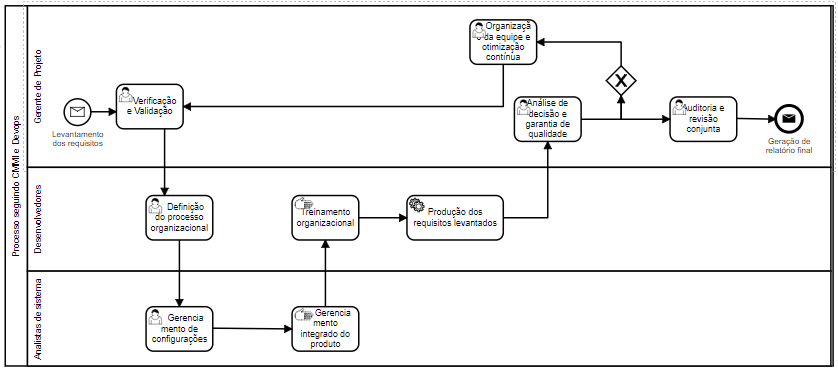
\includegraphics[scale=0.8]{processo-final(bpmn)}
\end{figure}

As etapas definidas para o processo foram:

 \begin{description}
	\item[Levantamento dos requisitos]: Etapa onde os requisitos e novas funcionalidades para a nova versão do software são levantadas e analisadas. Como o DevOps preza por uma comunicação maior de toda a equipe participam tanto os gerentes do projeto, desenvolvedores, designers, operadores de infraestrutura, etc.
	\item[Verificação e Validação]: Os requisitos discutidos são organizados e validados pela equipe para ser implementado.
	\item[Definição do processo organizacional] São relatadas as atividades de cada integrante e do desenvolvedor, tanto para o desenvolvimento de um novo software ou manutenções. Define atribuições genéricas e as responsabilidades do gerente em relação ao ciclo de vida do software. Descreve as atividades básicas para a criação e manutenção de uma infraestrutura adequada.
	\item[Gerenciamento de configurações]: Controle e manutenção da integridade dos itens do software ao longo de seu ciclo de vida.
	\item[Gerenciamento integrado do produto]: Garantir a integração de todos da equipe e que garanta que o produto de software esteja em conformidade com os requisitos e os planos estabelecidos.
	\item[Treinamento Organizacional]:  Aplicação de treinamento da norma ISO/IEC 12207, mostrando que a norma é adaptável entre seus processos como que com outras normas. Também é realizado uma dinâmica para fixar e estimular a prática DevOps.
	\item[Produção dos requisitos levantados]: Implementação das novas funcionalidades e geração de uma nova versão do software.
	\item[Análise de decisão e garantia da qualidade]: Determina se o software ou requisito atende ao uso específico proposto e verificação da garantia de qualidade do produto.
	\item[Organização da equipe e otimização contínua]: Etapa necessária caso a análise de decisão da equipe não seja positiva. Utilizado mecanismos para a resolução de problemas ou não conformidades por meio de um processo fechado utilizando-se de ações corretivas e também a organização da equipe para as correções.
	\item[Auditoria e revisão conjunta]: Prepara o ambiente para a realização de auditorias com ênfase no cumprimento dos requisitos de produtos e serviços. Além disso, define as atividades para avaliação da situação e de produtos, visando o uso e aceitação do cliente.
	\item[Geração de relatório final]: Geração das funcionalidades desenvolvidas, do andamento do processo e pontos positivos e negativos relatados durante o desenvolvimento. E também ocorre distribuição aos interessados sobre os registros e documentação produzida durante a execução.
\end{description}


\section{Risco}
Os riscos apresentados são:

\begin{enumerate}
	\item A não aceitação pelo cliente das novas funcionalidades desenvolvidas.
	\item A equipe não se adequar ao novo processo estabelecido
	\item O tempo e cronograma estabelecidos não serem cumpridos
	\item Perdas financeiras
	\item Aumento dos custos
	\item Perda de mercado
\end{enumerate}

\section{Plano de manutenção}
Para evitar problemas na empresa deve ser definido um programa de manutenção com métodos preventivos estabelecidas e com qualidade, caso algum equipamento ou servidor venha a apresentar problemas. 
O plano consistem em monitorar as partes do sistema regularmente e efetuar backups periódicos. Também é necessário ajustar ou trocar componentes em períodos predeterminados, testar os equipamentos com frequência e garantir um programa de prevenção tanto para equipe de desenvolvimento quanto para os clientes.

\section{Referências bibliográficas}

Exemplo: Redes de computadores, segundo \cite{t2013} é considerada..... Já \cite{kurose2010} apresenta uma versão...

Analisando os pressupostos de \cite{ref3} e \cite{ref4} concluimos que....


\renewcommand\refname{} %%Referências bibliográficas}  
\bibliographystyle{ieeetr}
\bibliography{referencias}  


\end{document}